\documentclass[../main.tex]{subfiles}
\begin{document}
\section{Introduzione}
Ciò che differenzia tutte le varie "ere" è l'attività che l'uomo era in grado di compiere.
\begin{itemize}
    \item \textbf{Età della pietra}:
    \begin{itemize}
        \item \textbf{Paleolitico}: 2.5 milioni di anni fa - 10.000 anni fa, pietra scheggiata 
        \item \textbf{Mesolitico}: 10.000 anni fa - 8.000 a.C., schegge piccole, agricoltura, arco freccia spago $\rightarrow$ agricoltura
        \item \textbf{Neolitico}: 8.000 a.C. - 3500 a.C., pietra levigata + legno + ossi
    \end{itemize}
    \item \textbf{Età del rame}: 3500 a.C. - 2300 a.C. forno ruota vetro ceramica
    \item \textbf{Età del bronzo}: 2300 a.C. - 1000 a.C., l'uomo impara a fare le leghe
    \item \textbf{Età del ferro}: 1300 a.C. - 470 d.C., ferro, arrivano le armi, ma il problema del ferro è la ruggine: nascono le operazioni di finitura per renderlo meno attaccabile dalla ruggine. Un altro problema del ferro è la necessità di temperature elevate.
    \begin{itemize}
        \item Età antica: 700 a.C - 400 d.C. mulino ad acqua per svolgere il lavoro che prima era svolto da animali da soma, primo sfruttamento dell'energia. Poi mulino a vento.
        \item Medioevo: 400 d.C. - 1450 d.C., scrittura molto importante per il know-how.
    \end{itemize}
\end{itemize}

\section{Tecnologia}
\begin{center}
    Dal greco: Trattato su un'arte.
\end{center}
\begin{itemize}
    \item Tecnologie preistoriche:
    \begin{itemize}
        \item Utensili di pieta + legno + materiali organici (zappa arco, ago, vasi)
        \item macchine di pietra, macine, azionate dall'uomo o da animali
        \item forni (a cumulo), stampi, macchine per filatura, telai
        \item metalli battuti + calore $\rightarrow$ resistenza
    \end{itemize}
    \item Tecnologie ellenistiche o alessandrine (Scrittura)
    \item Tecnologie dell'antica Roma: acquedotti (energia = gravità pendenza del 2\%; utensili = vasche di depurazione, ponti, dotti)
    \item Tecnologie da guerra: catapulte, specchi ustori, polvere "nera" - salnitro $KNO_3$, carbone vegetale e zolfo - Industria chimica
    \item Tecnologie di navigazione: scoperta dell'elettromagnetismo, bussola.
\end{itemize}
\subsection{Leonardo Da Vinci}
Tecninca arte-scrittura.
\begin{itemize}
    \item Meccanica: ingranaggi, macchine per fabbiricare viti, per levigare
    \item Tessile: 
    \item Militare
    \item Navale
\end{itemize}
\textbf{Rivoluzione scientifica}: fisica sperimentale e strumentale - misurazioni, esperienze\\
\textbf{Rivoluzione industriale}: 1750 - Acciaio e il vapore, pompe, biella-manovella. Moto rettilineo e moto rotatorio

\subsection{Motore a benzina}
Tecnologia meccanica.\\
\begin{figure}[h!]
    \centering
    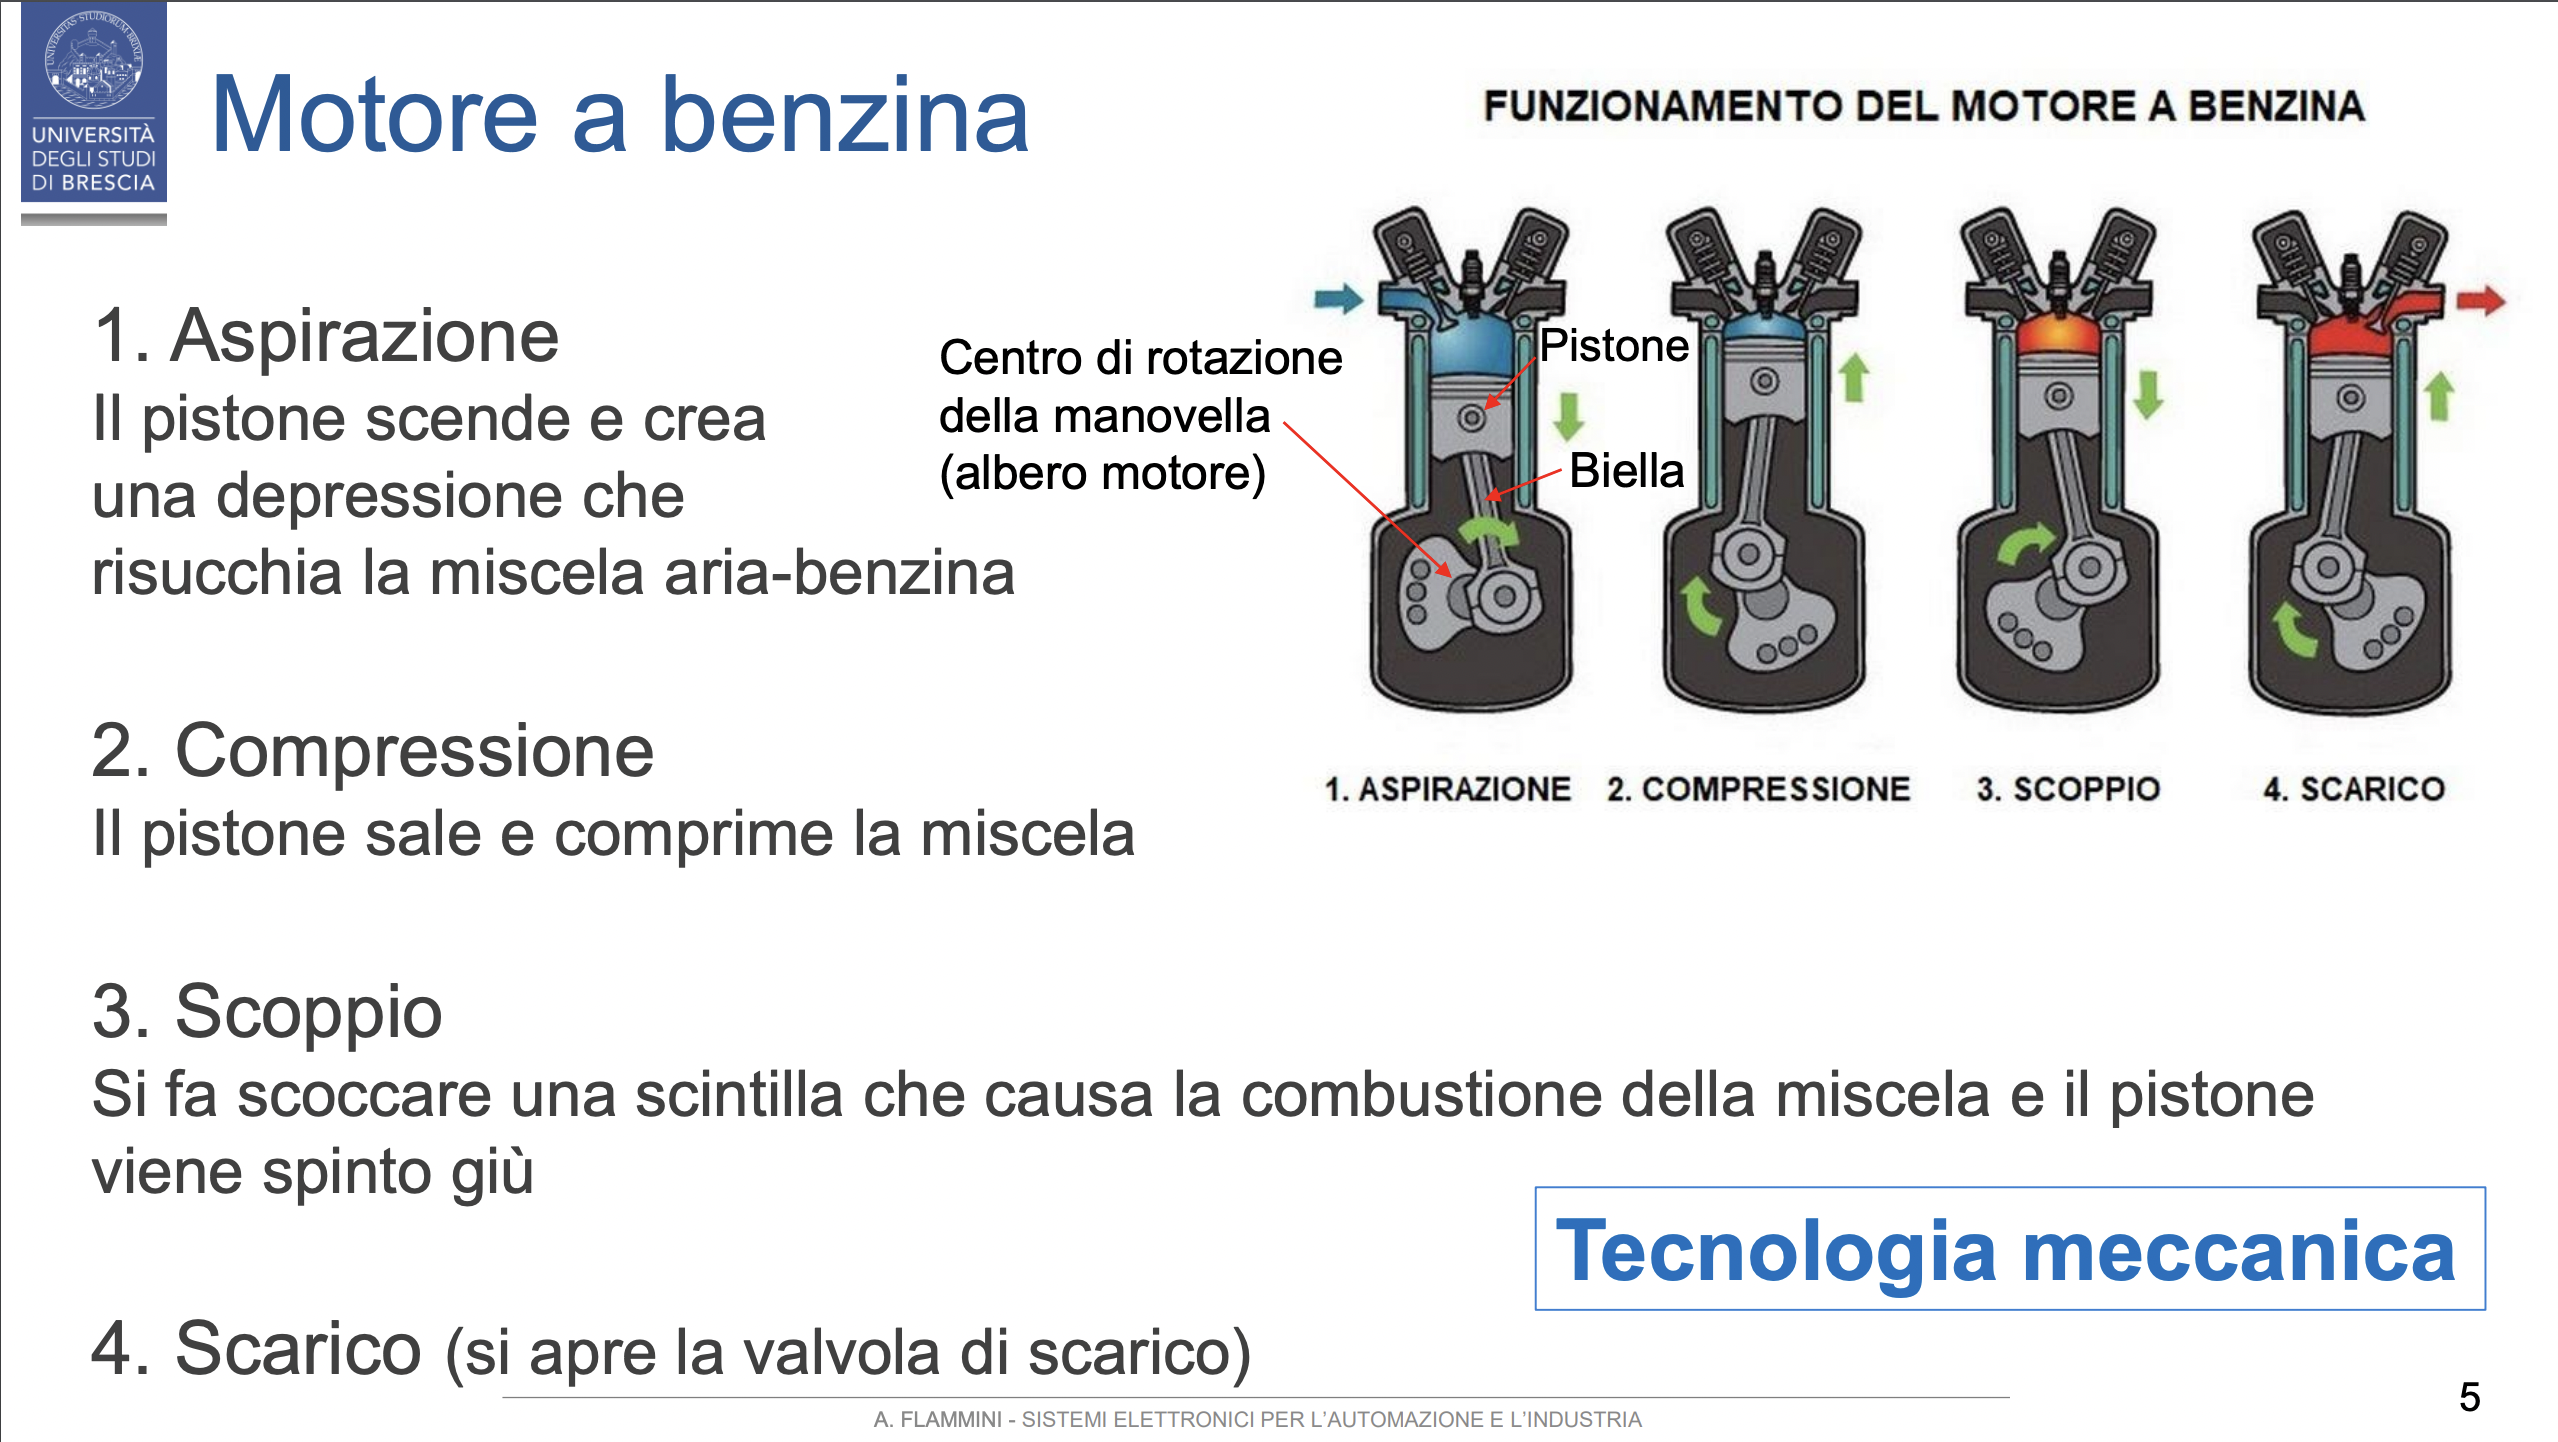
\includegraphics[width=0.7\linewidth]{banz.png}
    \caption{Motore a benzina}
\end{figure}

\subsection{Rivoluzioni industriali}
\begin{figure}[h!]
    \centering
    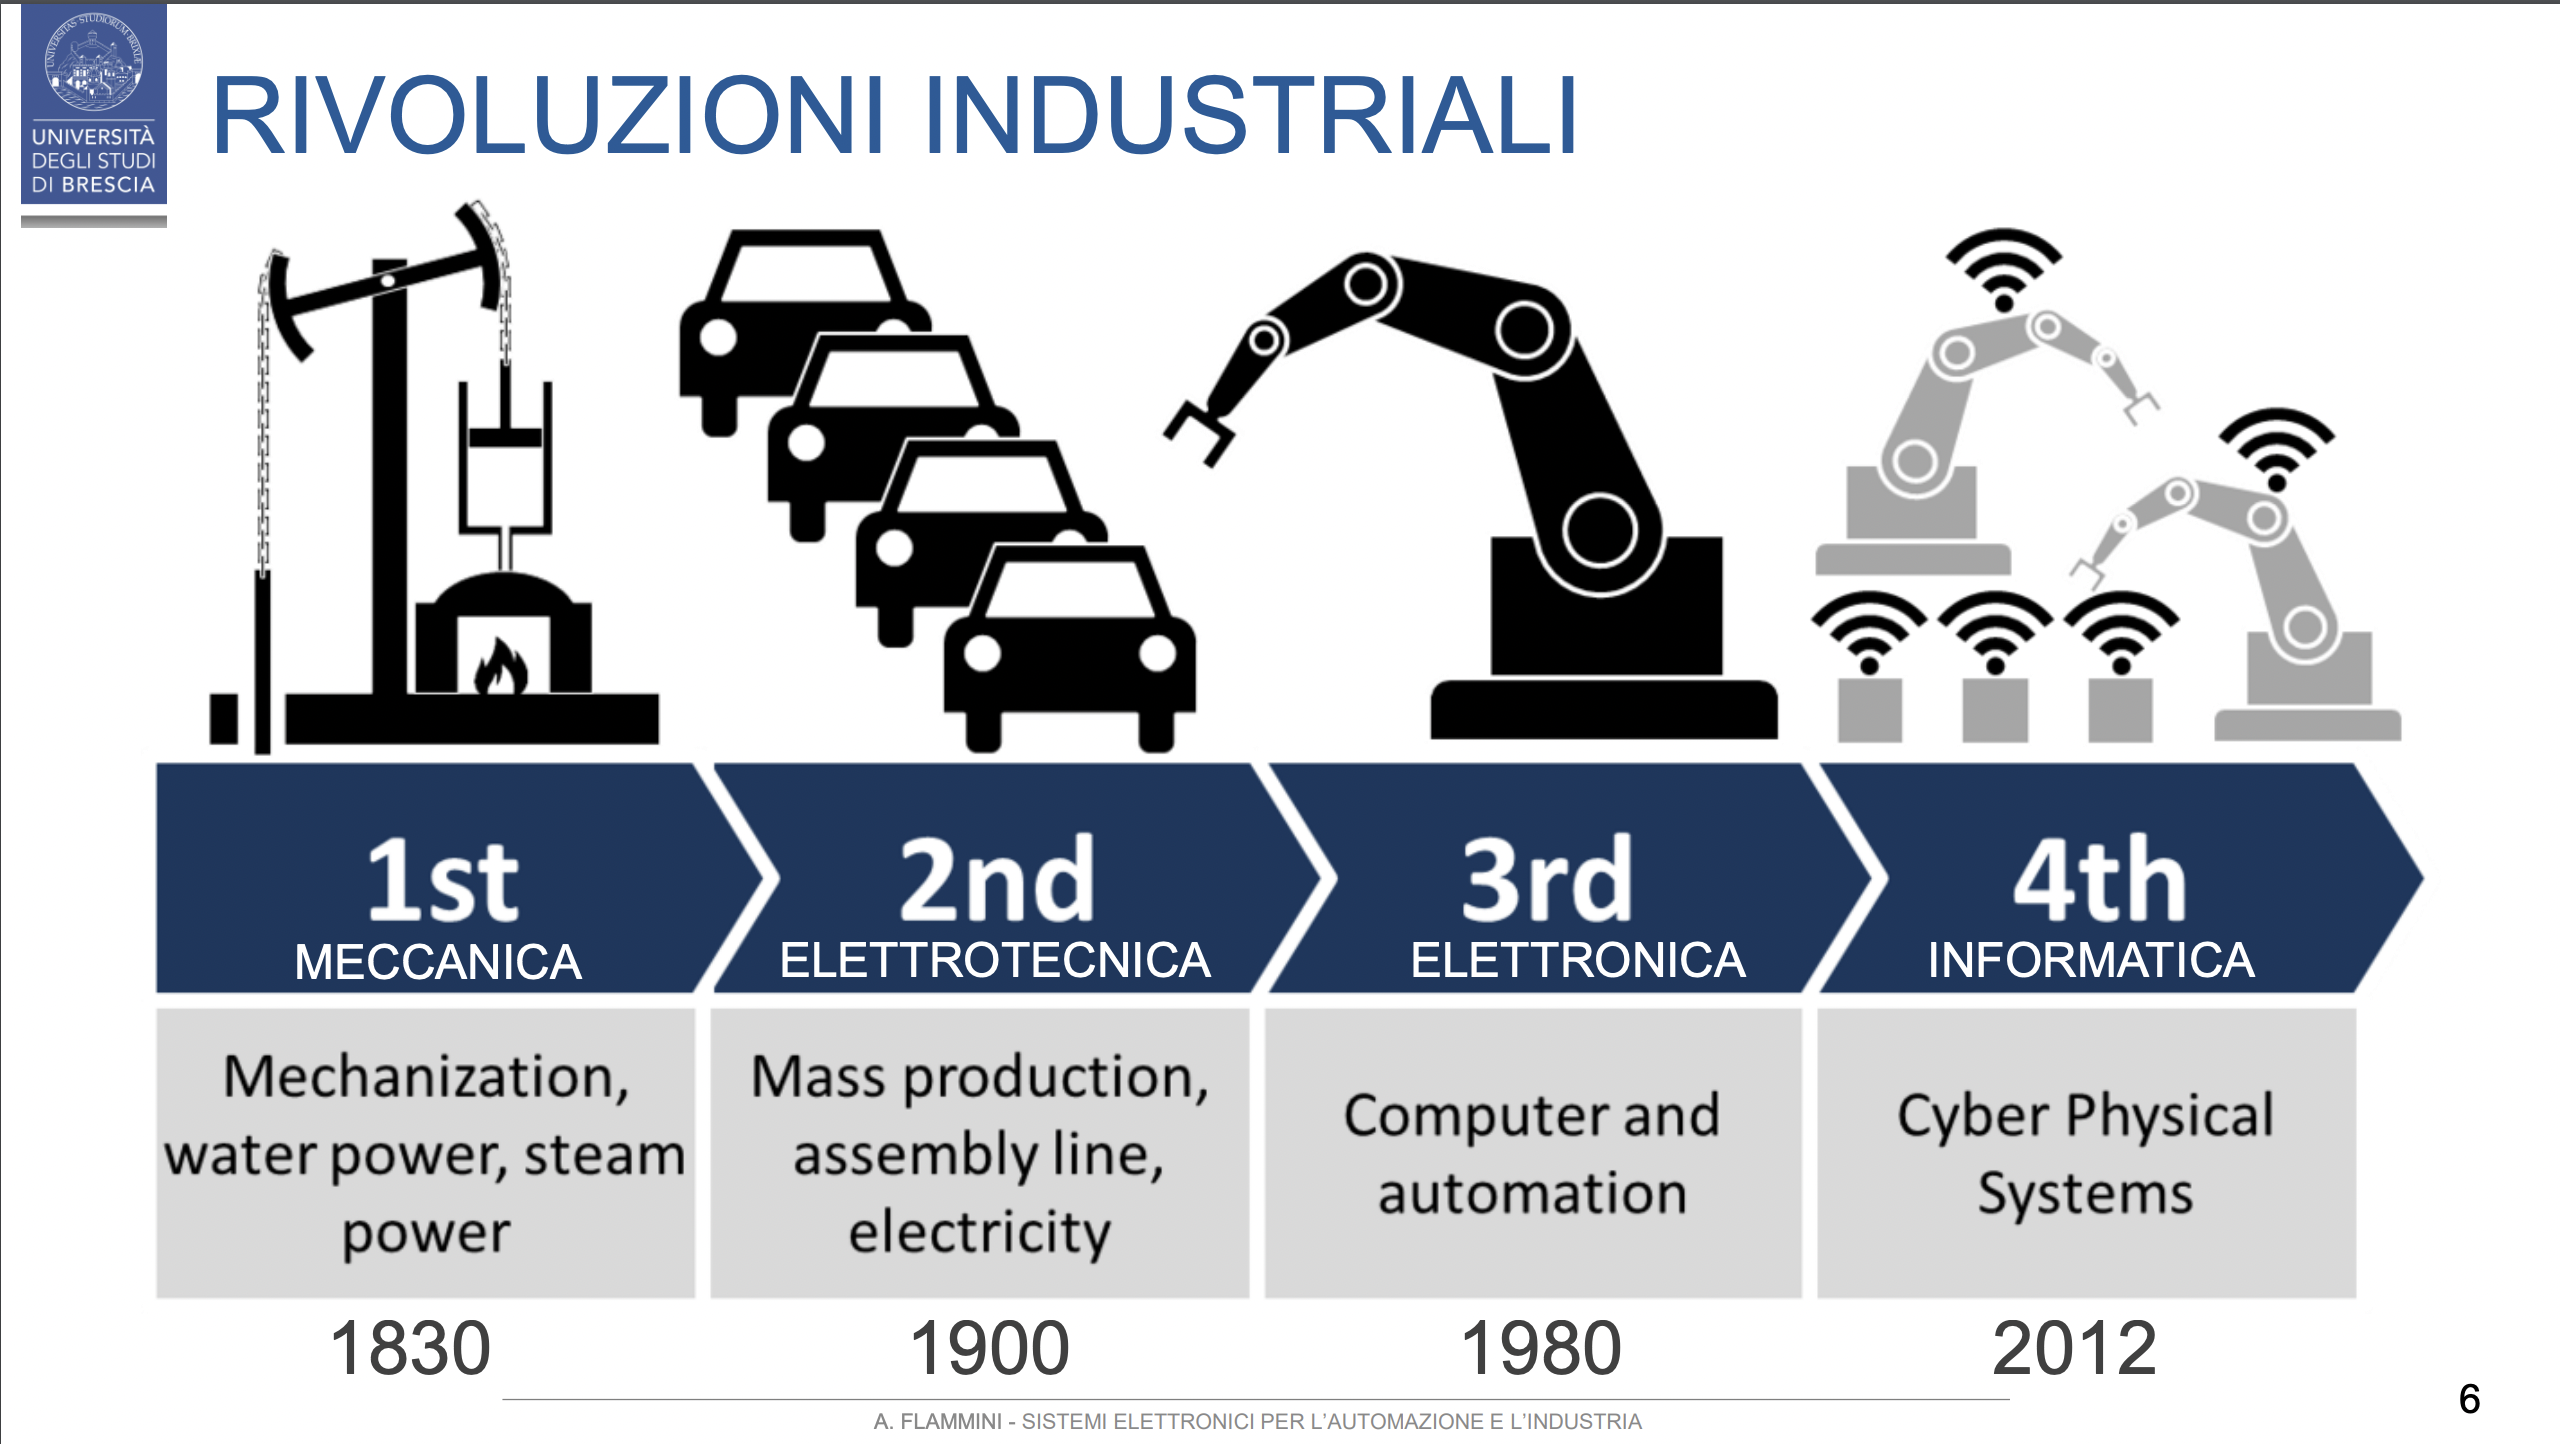
\includegraphics[width=0.7\linewidth]{riv.png}
    \caption{Rivoluzioni industriali}
\end{figure}
Energia muscolare $\rightarrow$ vento, energia naturale $\rightarrow$ forni $\rightarrow$ vapore $\rightarrow$ elettricità, con la quale si avvia la produzione di massa (elettrotecninca - fordismo) $\rightarrow$ elettronica (PLC), nato in Giappone con la Toyota $\rightarrow$ reti di comunicazione che permettono ai diversi controllori di comunicare tra di loro $\rightarrow$ informatica (controllo a distanza) $\rightarrow$ quinta rivoluzione industriale, rivolzione umano-centrica.

\subsection*{Classificazione a 3 assi dei sistemi di produzione}
\begin{itemize}
    \item \textbf{Asse del mercato}: modalità di vendita, su ordine (progetta, produci, assembla) per il magazzino (previsione)
    \item \textbf{Asse gestionale}: modalità di realizzazione del volume. Produzioni unitario su commessa, a lotti, continue. 
    \item \textbf{Asse tecnologico}: modalità di realizzazione del prodotto. \begin{itemize}
        \item Industria di base o di processo: produzione di energia, processi chimici, processi estrattivi. Industria che riguarda la distribuzione
        \item Industria di fabbricazione: produzione da materiali grezzi o semilavorati (\textbf{irreversibile} - trasformazione fisico-tecnica) e assemblaggio (tendenzialmente \textbf{reversibile}).
    \end{itemize}
\end{itemize}

\end{document}